\section{Оптимизации}
По подразбиране Rust компилра кода без никакви оптимизации и с много символи
които помагат за по лесното дебъгване на програмата. Когато компилираме кода
за употреба от нашите потребители, искаме нашата програма да е възможно
най-бърза и с най-малък размер. Но преди това трябва да кажем на компилатора
как по-точно искаме да бъде оптимизирана програмата. Това се случва като добавим
следните 5 реда в Cargo.toml [Фигура \ref{fig:optimization-config}].
\begin{itemize}
    \item strip - премахва символите за повечето дебъгване;
    \item opt-level - колко пъти компилатора да се пробва да оптимизира кода;
    \item lto - извършва оптимизации при свързването (linking) на всички библиотеки с програмата;
    \item codegen-units - колко паралени нишки да бъдат създадени за по-бързо компилиране, когато се използва само 1 нишка кода може да бъде оптимизиран по-добре.
\end{itemize}

\begin{figure}[!htb]
  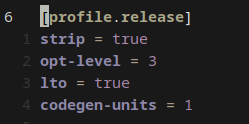
\includegraphics[scale=0.85]{optimization-config.png}
  \centering
  \caption{Допълнителни настройки за оптимизиране на кода}
  \label{fig:optimization-config}
\end{figure}

За да кажем на компилатора да компилира програвата с всички оптимизации, можем
да подадем --release флага на компилатора.
\begin{lstlisting}
cargo build --release
\end{lstlisting}

Разликата между двата файла е огромна. Не оптимизирания файл е цели 272
мегабайта, а оптимизирания едва 10 мегабайта [Фигура
\ref{fig:optimization-size}]. Освен птимизации за размер, Rust прилага и
оптимизации за време. 

\begin{figure}[!htb]
  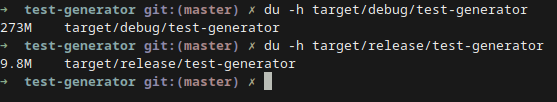
\includegraphics[scale=0.85]{optimization-size.png}
  \centering
  \caption{Разлика в размера при Debug и Release компилиране}
  \label{fig:optimization-size}
\end{figure}

Тестовете за време са извършени при 1000 итерации и времето е изчислено
следно-аретметично и като медиана. Средното времето за изпълнение пада от 20
милисекунди на по-малко то 2 милисекунди, а медианата от почти 43 милисекунди
на 3. Между двата начина за тестване, скороста на изпълнение се увеличава
повече от 10 пъти [Фигура \ref{fig:optimization-time}].

\begin{figure}[!htb]
  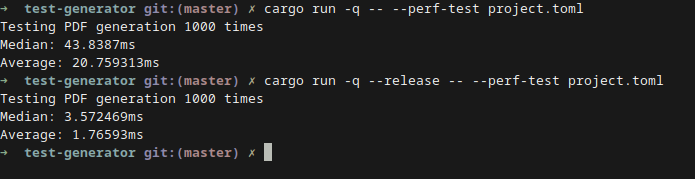
\includegraphics[scale=0.75]{optimization-time.png}
  \centering
  \caption{Разлика в скороста на изпълнение при Debug и Release компилиране}
  \label{fig:optimization-time}
\end{figure}
